\chapter{Study Management}

In this module the \entitytarget{Study} aggregate is used to configure a
study. It defines the valid types of specimens that can be collected, when they
are to be collected from participants, and how the collected specimens are
processed. This aggregate is made up of the entities and value objects shown in
the figure below.

This section first describes the study aggregate and then defines the commands
it handles.

\begin{figure}[h]
  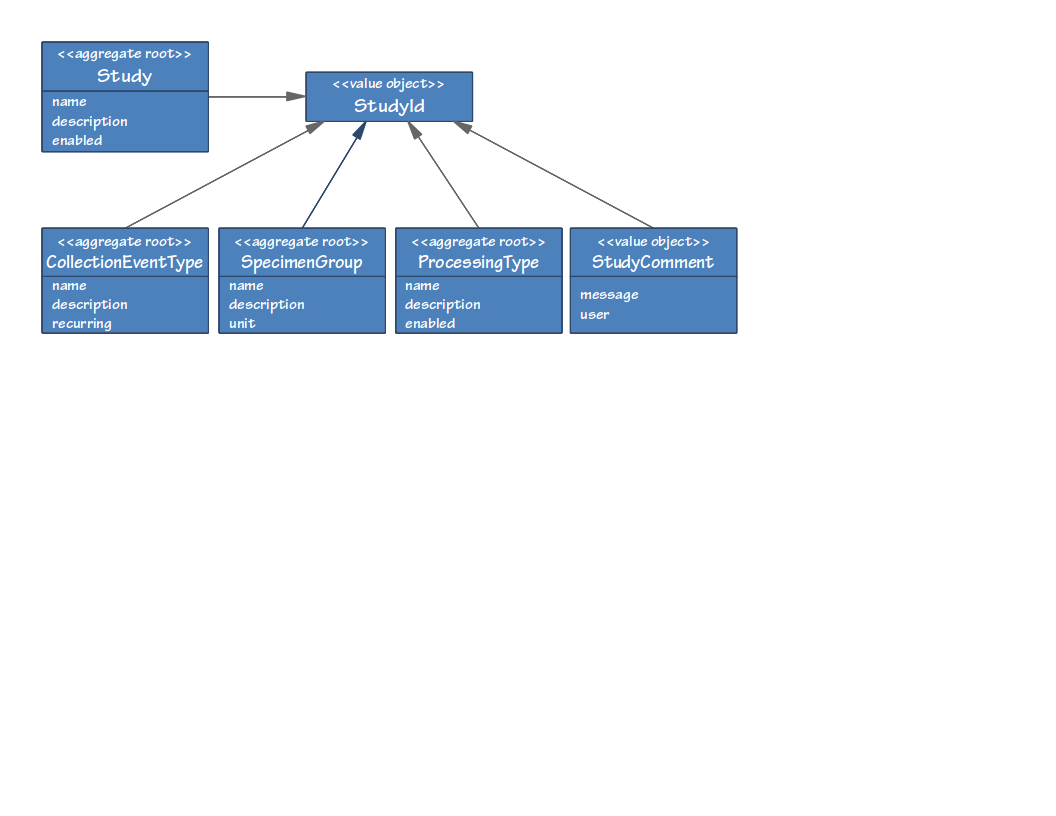
\includegraphics[trim={9mm 85mm 36mm 9mm}, clip,
    width=1\textwidth]{images/study-aggregate}
  \caption{Study aggregate}
  \label{fig:study-aggregate}
\end{figure}

\subsection*{Study}

Represents a collection of participants and specimens collected for a
particular research study. The study name is a short descriptive name that is
usually an acronym used for quick identification. The description contains text
used to give more details on the name and is usually the words that make up the
acronym.

A study can be enabled or disabled. When disabled, changes to its configuration
are possible but patients and specimens cannot be added. When enabled, no
further configuration changes are allowed, and participants and specimens can
be added.

A study may have one or more comments assigned to it during it's lifetime.

\subsection*{SpecimenGroup}

This entity is used to record the specimen types used by the study.  It records
wwnership, summary, storage, and classification information that applies to an
entire group or collection of \entitylink{Specimen}s. It is used to specify
specimens collected from participants, and the specimens that are processed
from them.

The anatomical source, preservation medium and specimen type are defined using
other value objects discussed in Section \ref{sec:specimen-group}.

\subsection*{CollectionEventType}

A classification name, unique to the \entitylink{Study}, for a visit by study
participants. For specimen collection to be allowed on a study, at least one
collection event type must be defined. Each collection event type has one or
more specimen groups (see Section \ref{sec:collection-event-type}).

\subsection*{ProcessingType}

Describes a regularly performed specimen processing procedure with a unique
name (unique to the \entitylink{Study}). There should be one or more associated
\entitylink{SpecimenLinkType}s that (1) further define legal procedures and (2)
allow recording of procedures performed on different types of
\entitylink{Specimen}s.

\subsection*{StudyAnnotationType}

Annotations allow further customization of a study and record supplementary
information. Annotations can be used with the following entities: collection
event types (Section \ref{sec:collection-event-type}), processing events
(Section \ref{sec:processing-type}), and participants (Section
\ref{sec:participant-annotations}).

\subsection*{StudyComment}

The comment contains a message and the user that added the comment. The date
and time the comment was made is recorded as meta data.

\section{SpecimenGroup Details}
\label{sec:specimen-group}

The \entitytarget{SpecimenGroup} entity is
composed of other value objects as shown in Figure
\ref{fig:specimen-group}. \entitylink{SpecimenGroup} entities are accessed via
the \entitylink{Study} aggregate.

\begin{figure}[h]
  \centering
  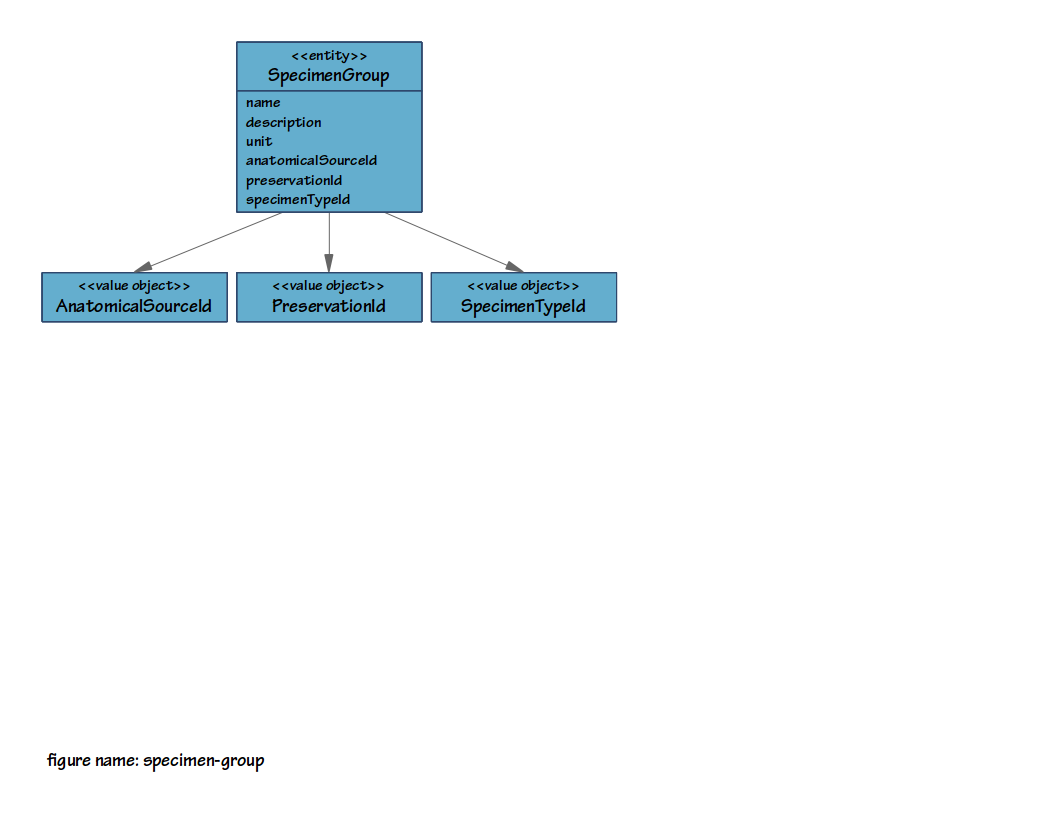
\includegraphics[trim={9mm 162mm 80mm 9mm}, clip,
    width=1\textwidth]{images/specimen-group}
  \caption{SpecimenGroup entity}
  \label{fig:specimen-group}
\end{figure}

\subsection*{AnatomicalSourceId}

The ID belonging to a \valobjlink{AnatomicalSource} which is a standardized set
of regions from a \entitylink{Participant} \emph{where} a \entitylink{Specimen}
is collected from. Potential examples include: colon, ear, leg, kidney, etc.

\subsection*{PreservationId}

The ID belonging to a \valobjlink{Preservation} value object which describes
how a \entitylink{Specimen} should be preserved/stored by describing
temperature requirements ($^\circ$C), as well as a preservation method (see
\valobjlink{PreservationType}).

\subsection*{SpecimenTypeId}

The ID belonging to a \valobjlink{SpecimenType} which is standardized set of
classifications that describe \emph{what} a \entitylink{Specimen} is. Potential
examples include: urine, whole blood, plasma, nail, protein, etc.

\section{CollectionEventType Details}
\label{sec:collection-event-type}

A collection even type can be configured to collect one or more specimens using
\entitylink{SpecimenGroupCollectionEventType}. Also, it can be configured to
record one or more annotation types using
\entitylink{CollectionEventTypeAnnotationType}. These associations are shown in
Figure \ref{fig:collection-event-type}.

\begin{figure}[h]
  \centering
  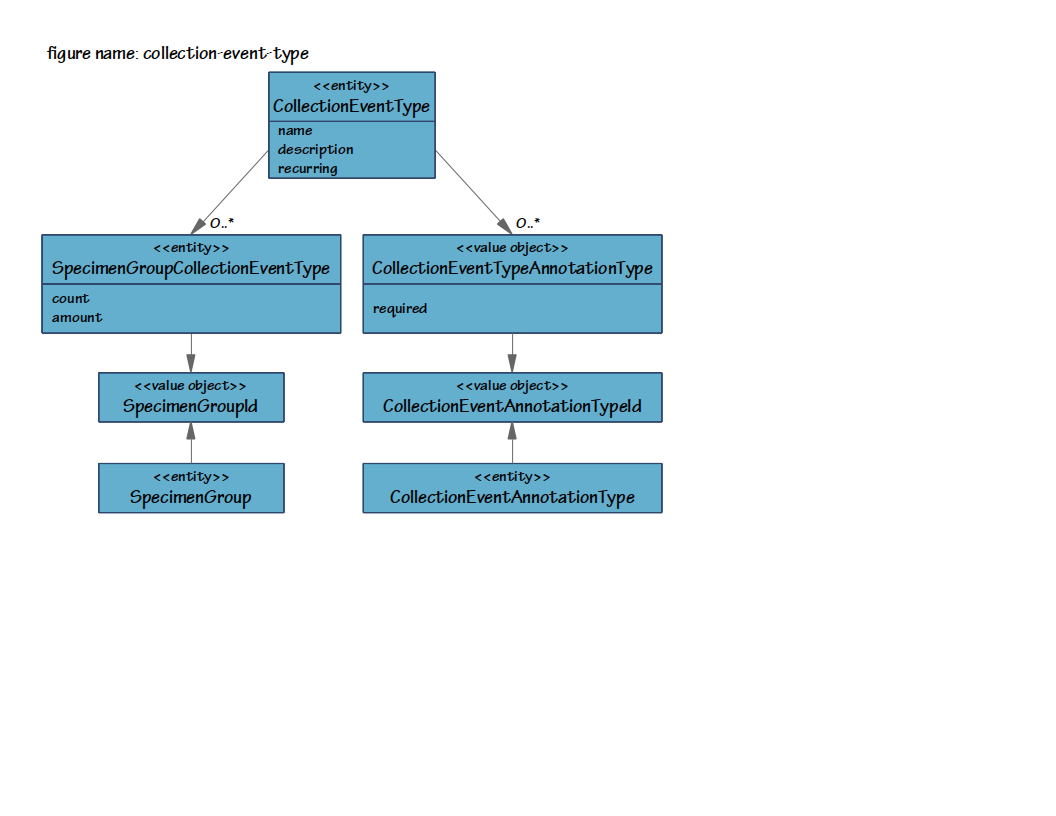
\includegraphics[trim={9mm 45mm 96mm 9mm}, clip,
    width=0.8\textwidth]{images/collection-event-type}
  \caption{Details for the CollectionEventType entity}
  \label{fig:collection-event-type}
\end{figure}

\subsection*{SpecimenGroupCollectionEventType}

\valobjtarget{SpecimenGroupCollectionEventType}s are used to
define which types of specimens (i.e. which \valobjlink{SpecimenGroup}s) need
to be collected with a type of collection event.

The \texttt{count} specifies how many specimens are to be collected. The
\texttt{amount} is the amount of substance that is expected in each collected
specimen, or null if there is no default amount.

\subsection*{CollectionEventTypeAnnotationType}

One or more \valobjtarget{CollectionEventTypeAnnotationType} are used to record
the annotation types to be recorded with a collection event type. When required
is set to true the annotation value is not allowed to be empty.

\section{ProcessingType Details}
\label{sec:processing-type}

A processing type can be configured to process one or more collected specimens
using \valobjlink{SpecimenLinkType}. Individual specimen link types within the
processing type can also be configured to record one or more annotation using
\valobjlink{SpecimenLinkTypeAnnotationType}. Figure \ref{fig:processing-type}
provides more details for the processing type entity.

\begin{figure}[H]
  \centering
  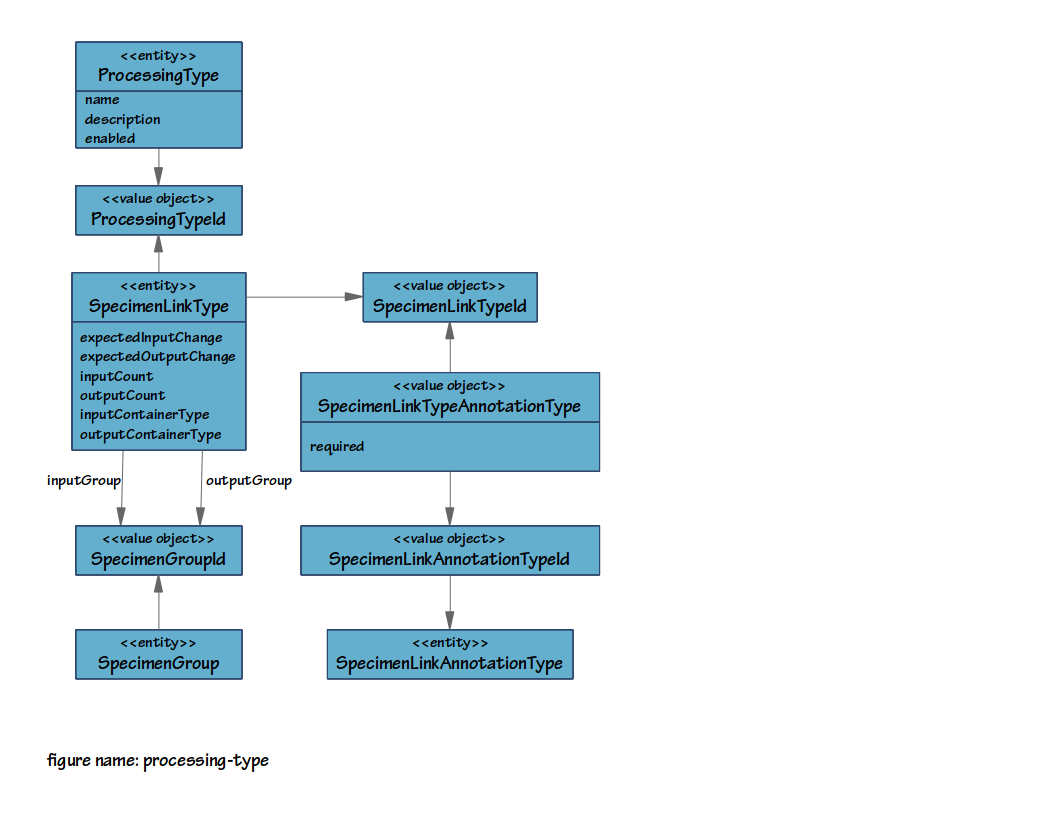
\includegraphics[trim={9mm 38mm 45mm 9mm}, clip,
    width=1\textwidth]{images/processing-type}
  \caption{Details for the ProcessingType entity.}
  \label{fig:processing-type}
\end{figure}

\subsection*{SpecimenLinkType}

 \valobjtarget{SpecimenLinkType}s are assigned to
a processing type, and used to represent a regularly performed processing
procedure involving two \entitylink{Specimen}s: an input, which must be in a
specific \valobjlink{SpecimenGroup}, and an output, which must be in a specific
\valobjlink{SpecimenGroup}.

The \texttt{expectedInputChange} is the expected amount (decimal value) to be
removed from each input. The \texttt{expectedOutputChange} is the expected
amount to be added to each output. The expected input and output change values
can be zero.  The counts in \texttt{inputCount} and \texttt{outputCount} are
the number of expected and resulting specimens, respectively, when the
processing is carried out. A value of zero for output count implies that the
count is the same as the input count. The specimen container type that holds
the input specimens is given in \texttt{inputContainerType}. The specimen
container type that the output specimens are stored into is given in
\texttt{outputContainerType}. If specifying the container types is not required
for one or both of these fields they can be assigned the \texttt{null} value.

To avoid redundancy, a specimen link type may exist only once for a given input
and output specimen group.

\subsection*{SpecimenLinkAnnotationType}

Specimen link annotations are defined using
\valobjtarget{SpecimenLinkAnnotationType}. One or more of these can be defined
for the study.

\subsection*{SpecimenLinkTypeAnnotationType}

A \valobjtarget{SpecimenLinkTypeAnnotationType} is used to tie the specimen
link annotation types to a specimenlink type. \texttt{required} is set to
\texttt{true} the annotation value is not allowed to be empty.

\section{Participant Annotations}
\label{sec:participant-annotations}

\section {Study Aggregate Commands}
These are the commands used to configure a study.

\subsection*{StudyCreateCommand}

Used to create a study. The arguments are: \texttt{name (String)} and
\texttt{description (String)}. The name used to refer to the study and is
usually an acronym. The description describes the study and is usually the
words that make up the acronym.

\subsection*{StudyUpdateCommand}

Used to create a study. The arguments are: \texttt{studyId (String)},
\texttt{name (String)} and \texttt{description (String)}. The studyId is the
unique identifier for the study. The name contains the updated name or the
current name if no update is required. The description contains the updated
description or the current description if no update is required.

\subsection*{StudyEnableCommand}

Used to enable a study. Once enabled the study is ready to collect and process
specimens from participants. The single argument is \texttt{studyId (String)}
which is the unique identifier for the study.

\subsection*{StudyDisableCommand}

Used to disable a study. Once disabled the study can no longer collect and / or
process specimens from participants. The single arguments is \texttt{studyId
  (String)} which is the unique identifier for the study.

\subsection*{CreateSpecimenGroupCommand}

Used to create a specimen group in a study. The arguments are: \texttt{studyId
  (String)}, \texttt{name (String)}, \texttt{description (String)},
\texttt{anatomicalSourceId (String)}, \texttt{preservationId (String)}, and
\texttt{specimenTypeId (String)}. The studyId is the unique identifier for the
study. The name describes the specimen group. The description provides more
details for the speciment group.  The anatomicalSourceId is used to identify
anatomical source on the participants whre this group belongs to.  The
preservationId is used to record how this group is stored.  The specimenTypeId
identifies the type of specimens contained in this group.

\subsection*{DeleteSpecimenGroupCommand}

Used to delete a specimen group from the study. The arguments are:
\texttt{studyId (String)} and \texttt{specimenGroupId (String)}. The studyId is
the unique identifier for the study. The specimenGroupId is the unique
identifier for the specimen group.

